\documentclass[11pt]{article}
\pagestyle{headings}

\usepackage{fullpage}
\usepackage{graphicx}
\usepackage{sidecap}
\usepackage{subfig}
\usepackage{float}


\title{Tweet District Design Document}
\author{Victor Frolov}
\graphicspath{ {images/} }


\begin{document}
\maketitle

\section{Introduction}
Tweet District is an app that lets you find and interact with hundreds of tweets in your area (or any location of your choosing), and provides a way to find out about parties, local events, sales, promotions, and job hirings, and it's all shown on a map. Although it is currently a web app, it's use would be far greater on a mobile device. The purpose of this paper is to come up with a dream interface for this app, and use it as a guide during future development. Interaction design principles and theories are imperative to its development, and will range from usability measures, mental models, and many others.


\section{Landing Page}
Once a user downloads and opens the app, they will be greeted with a landing page with the logo, and app name that takes up a third of the screen. There will be one large button that allows the user to login to their existing twitter account (which will allow them to interact with the tweets, such as retweeting, sending direct messages, etc). Below the button will simply be clickable text that says "Use as Guest", allowing users to use the app without a twitter account. The logo, app name, button and text will be over a background color that will stay true to the app's theme. The background color will have opacity, and behind it there will be animations of users tweeting, partying, and shopping. Please see figure~\ref{fig:loginMock}.

\begin{figure}[H]
    \centering
    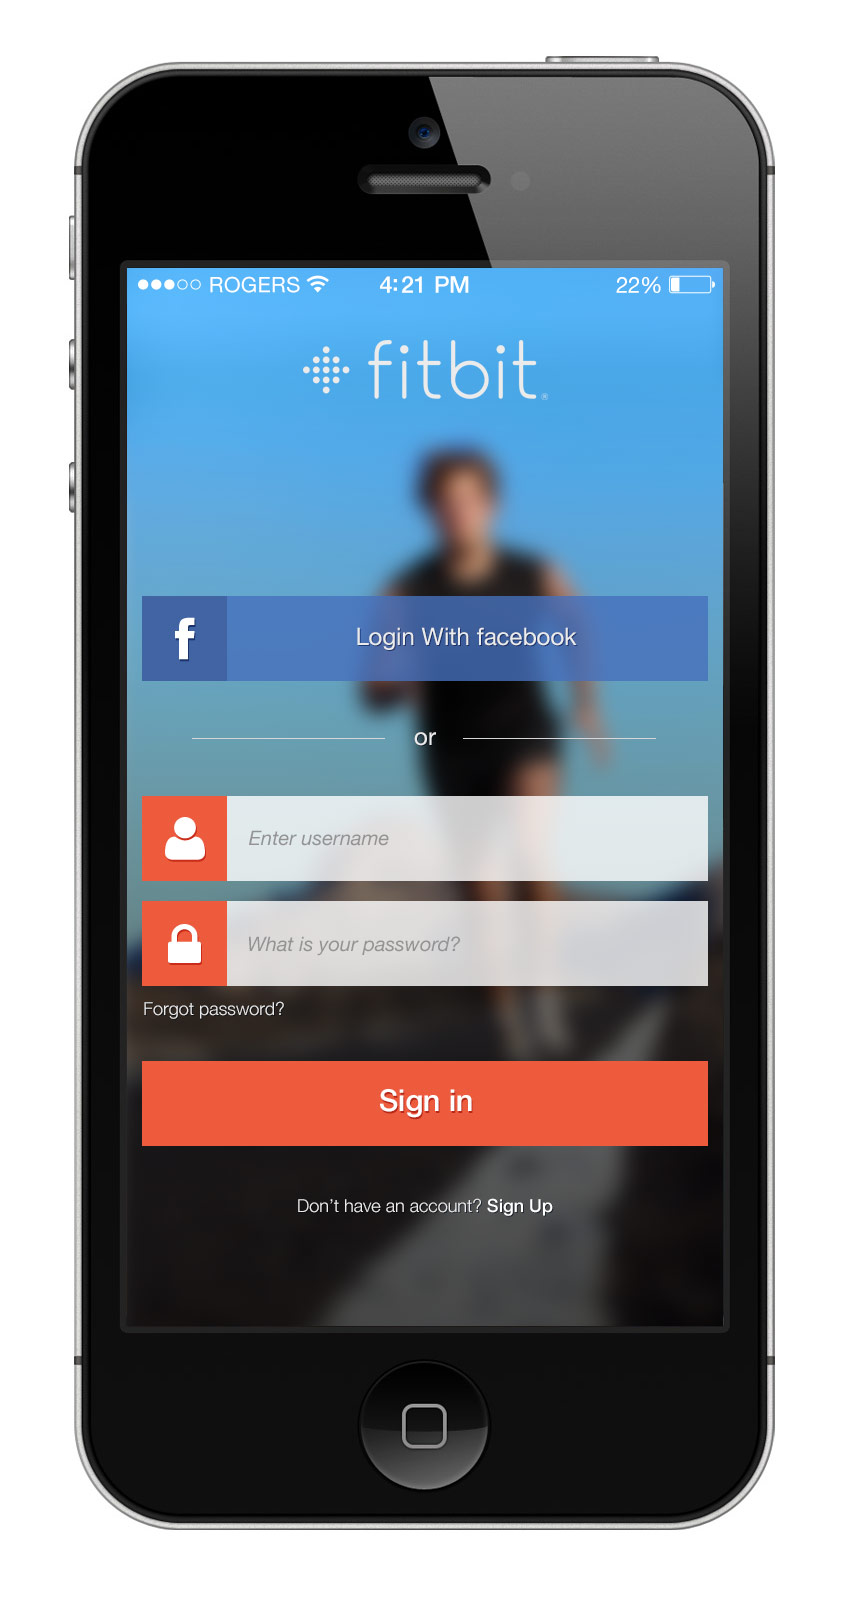
\includegraphics[width=7cm]{loginIdea}
    \caption{Landing/Login Page Example}  
    \label{fig:loginMock}          
\end{figure}

The "Login with Facebook" would be moved down to the "Sign in" location, and all other boxes and buttons would be removed. Login with Facebook would be changed to Twitter, and below it there would be the aforementioned text of "Use as Guest". The Fitbit logo and Fitbit name would be of course replaced with the Tweet District Logo and Tweet District name.


\section{Main Functionality}
The app's main functionality can be broken up into three sections:
\begin{itemize}
\item Searching
\item Displaying the tweets on a map
\item Displaying the tweets in an ordered fashion that is useful
\end{itemize}

Once a user either logins to their Twitter account, or continues as guest, they would be greeted with the search page. All pages, including the search page, would have a navigational dock with buttons on the bottom, like in iOS's native Podcast app. Please see Figure~\ref{fig:navButtons} below.

\begin{figure}[H]
    \centering
    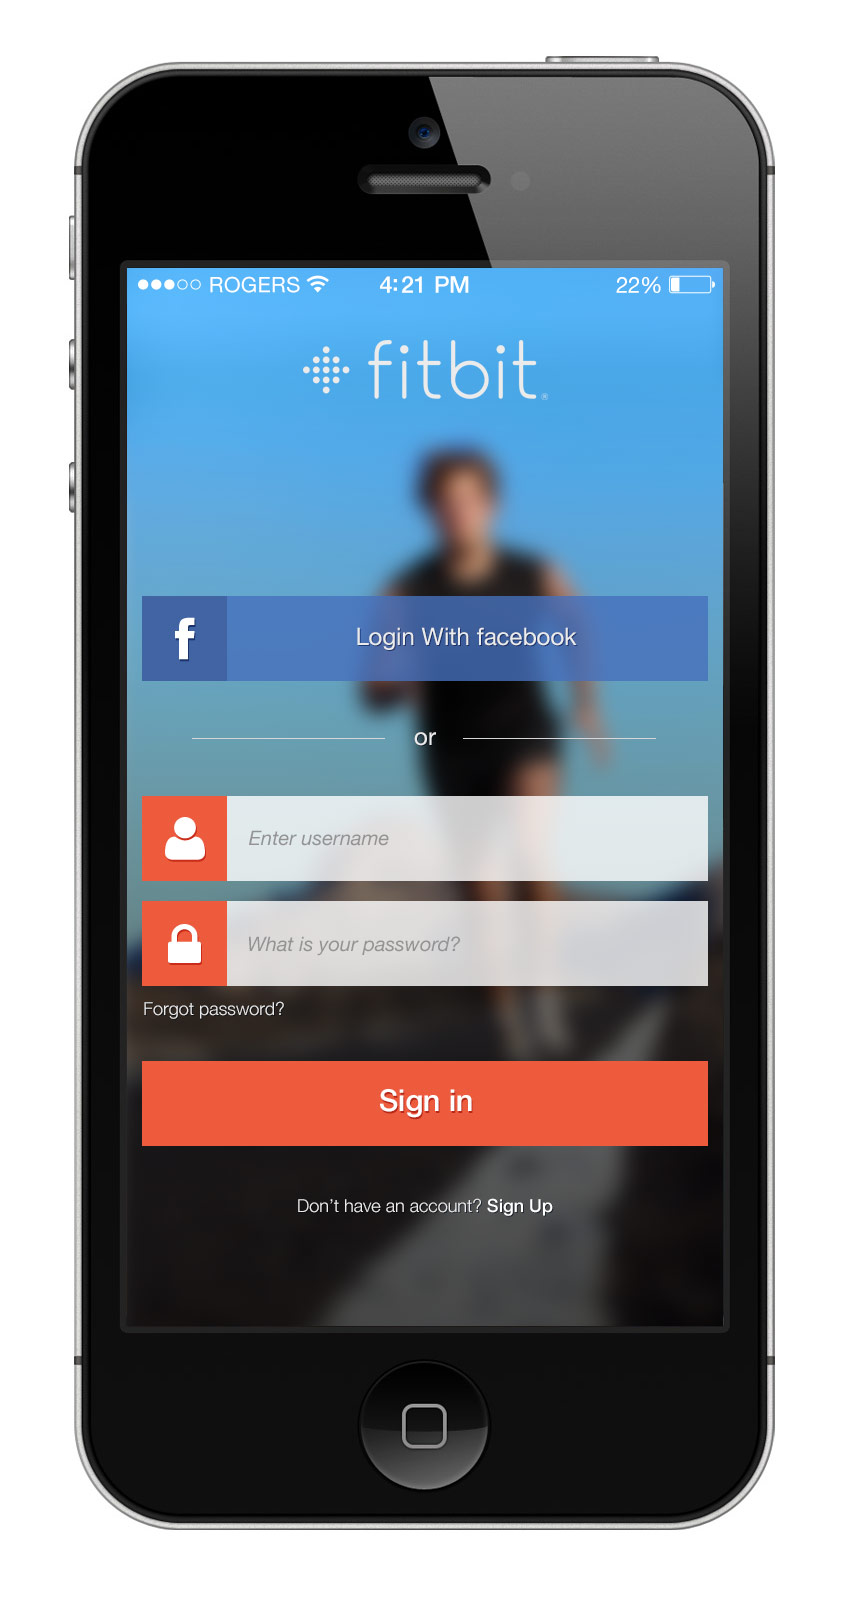
\includegraphics[width=7cm]{loginIdea}
    \caption{Navigational Buttons at the bottom of the Page}
    \label{fig:navButtons}                
\end{figure}


\subsection{Searching}
Before diving into the search functionality, it is important to note that all of the suggestions and current limitations are directly correlated to the usability metric of efficiency. The process of searching should be quick, simple and almost instantaneous, with optional extra steps for extra precision and only if the user demands it. It should not be forced upon them.

\subsubsection{Simplified Search}
When I tried using the app on my mobile device when I was out and about with some friends, we found that there were a few issues impeding us from having a great experience. The first issue was having to type in a search word, check the current location box, and clicking search each and every single time we tried looking up something around us. See Figure~\ref{fig:SearchSimple}.

\begin{figure}[H]
    \centering
    \subfloat[Current Search Appearance]{{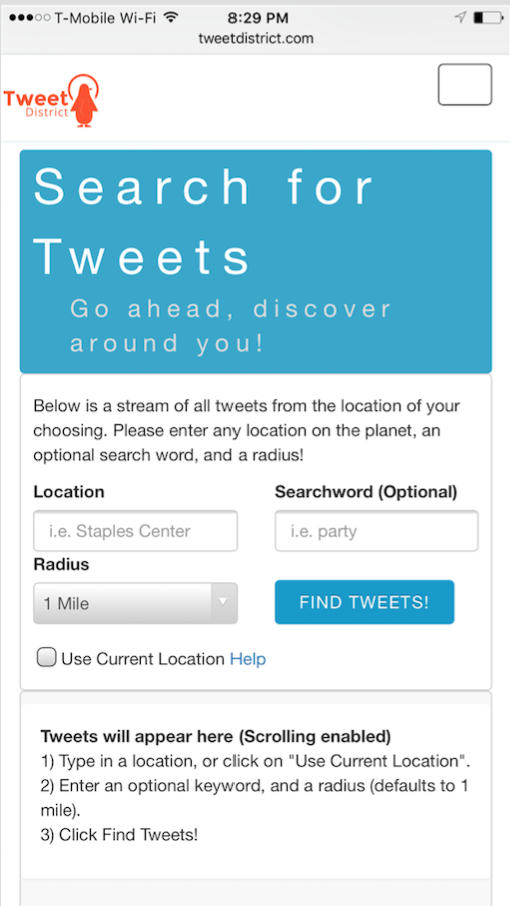
\includegraphics[width=7cm]{currentSearch} }}
    \qquad
    \subfloat[Simplified Search Appearance]{{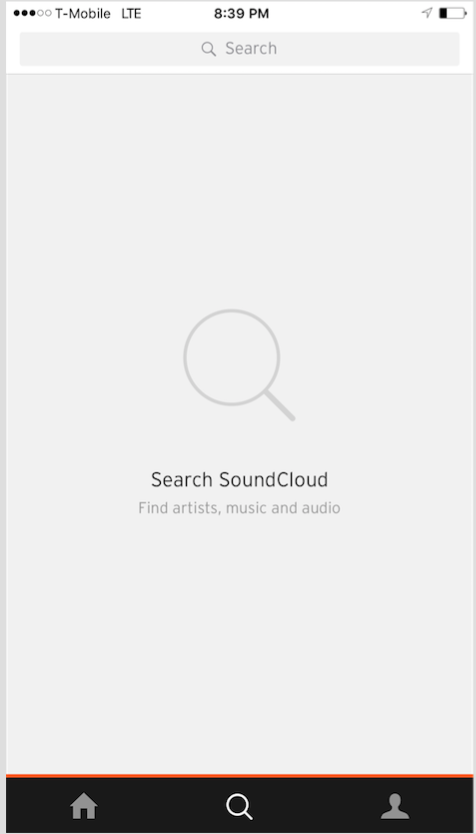
\includegraphics[width=7cm]{newSearch} }}
    \caption{Old Search and New Search Template}
    \label{fig:SearchSimple}          

\end{figure}

In order to overcome the first hurdle of having to repetitively do a series of steps (we tried looking up about 10 keywords to find events around us, and although it ultimately worked, the process was arduous), a simplified search, as in figure~\ref{fig:SearchSimple} (b), would be ideal. It would be preset to search a certain radius from the user's current location. That way they simply just type in a word or sequence of words, and hit search. 

\subsubsection{Advanced Search}
Since the app is all about searching, it is important to have advanced search still available. Text near the top that says "More Search Options", once pressed, would animate the app to swipe to the right, similar to Yahoo Fantasy Football's top left button. See Figure~\ref{fig:searchTemplate}.

\begin{figure}[H]
    \centering
    \subfloat[Before button was pressed]{{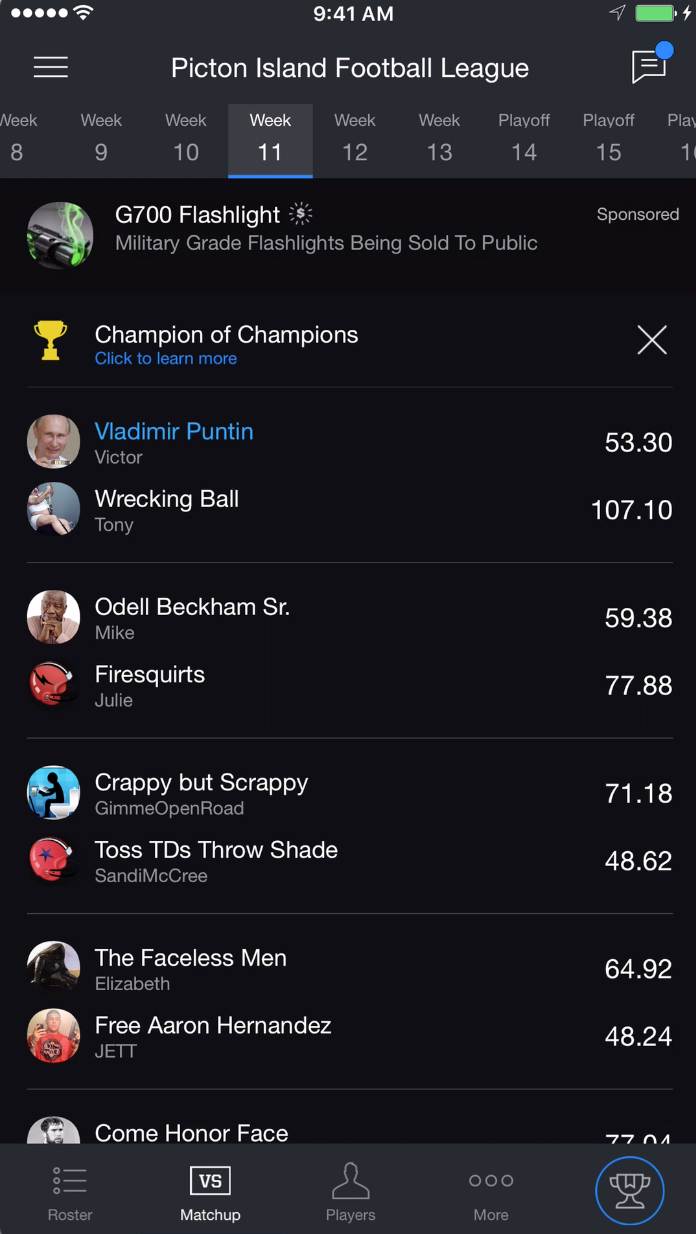
\includegraphics[width=7cm]{beforeSearch} }}
    \qquad
    \subfloat[After button was pressed]{{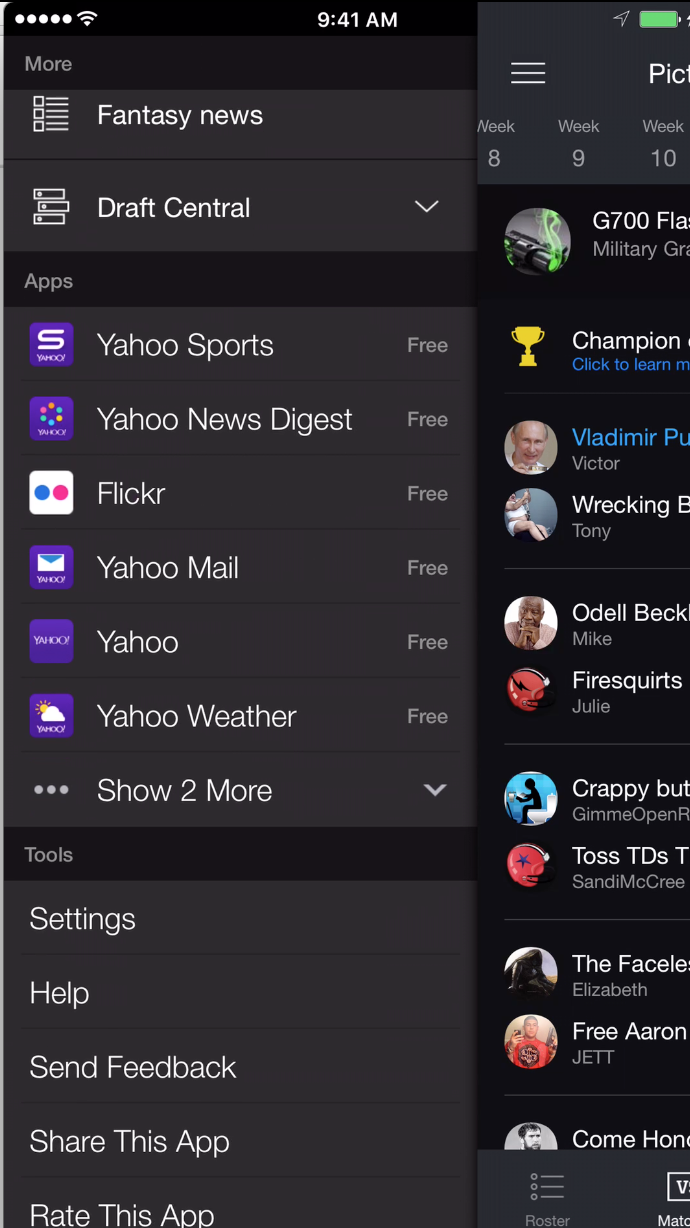
\includegraphics[width=7cm]{afterSearch} }}
    \caption{Advanced Searching}
    \label{fig:searchTemplate}
\end{figure}

So before the button was pressed, the search tab would simply look like Figure~\ref{fig:SearchSimple} (b), and after the button is pressed, it would slide everything on the screen to the right, and would look close to what Figure~\ref{fig:searchTemplate} (b) looks like. But of course, instead of displaying Yahoo information, it would show optional fields such as: custom radius, custom location (using geocoding and geodecoding), excluding certain users (this was a small issue where sometimes a user would tweet 20 times about the same event), enabling predefined searches, searching within a date range (so that a tweet from a few weeks ago that is no longer relevant doesn't show up), only displaying one tweet per user and excluding words and hashtags. The ability to save what the user input and make it become the "default" search should also be implemented. That way if the user always looks for "party" within a 3 mile radius of a specific location, they can do that with a single tap. Tapping on show less would slide the search back onto the screen, and would again look like figure~\ref{fig:SearchSimple} (b) above. The purpose of the animation is to draw attention to what is changing. 

\subsubsection{Deleting/Saving Search Results}
The ability to flick tweets that are of no interest should also be implemented. That way, if a user gets 100 tweets back from their search, if it is of no interest to them, they can swipe it left, which would not only remove the tweet from the list, but also remove a marker on the map associated to it. On the other end of the spectrum, they should be able to save tweets so that they can interact with them later, by swiping right. This would be saved and found under their "profile" tab. That way, they can at a later time share the tweet with friends, retweet it, direct message the user, or simply save it for whatever reason they want. Visually, this would look identical to the process of deleting or archiving mail on most mail apps, and would be accompanied by two different noises for each action. See Figure~\ref{fig:swipeDelete}.

\begin{figure}[H]
    \centering
    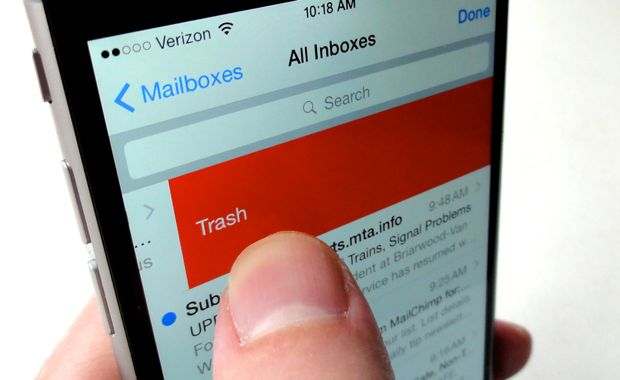
\includegraphics[width=7cm]{swipeDelete}
    \caption{Swiping to delete}
    \label{fig:swipeDelete}
\end{figure}

In case it is not obvious, as the user swipes, the entire box that contains the tweet would slide in a color (red or blue, depending on which action is occuring), and the more they swipe, the more the color slides in, until they finally reach the edge of the screen, on release, the tweet would be deleted/saved.

\subsubsection{Predefined Searches}

One final feature, which again would be to streamline searching, would be predefined searches. The user enables "predefined searches", in the advanced search options. This would then turn the search bar into a dropdown list of predefined searches. So, for example, if they were to select "party" in the dropdown list and hit search, it would automatically search the API for multiple keywords predefined by the app. Twitter's API allows the use of "OR" to string together multiple searches, so a potential combination could be "party OR frat OR houseparty OR happyhour OR bar OR club". Of course, custom predefined searches should also be implemented so that a user can look up series of words without having to type them fully out each time they do a search.



\subsubsection{Twitter's API Get/Searches Limitations}

As excellent as Twitter's API is, it has some limitations from Tweet District's perspective. They have the ability to ignore an ID's tweets, but, the ID must be known beforehand. Unfortunately, Twitter does not have the ability to cap or ignore users that have posted more than "x" tweets on a specific topic. This is a problem because, Twitter allows up to 100 tweets to be returned, and if there is a user spamming a certain topic, there is no clean way to ignore their tweets. One way would be to simply keep track of unique user ID's, and once there is repetition, to not append that tweet to the body, but of course, this would cause less than 100 tweets to be displayed. So if a user posted 60 times, and there was a total of 100 tweets, only 40 tweets would be displayed. A workaround would be to make an initial call, track the amount of unique ID's, and if a user, for example, has tweeted more than 5 or 10 times on a topic, to then do a second search, and ignore specifically his username in that search, for a more unique return.


\subsection{Map}
Another was that, since the map takes almost the full screen, scrolling to and away from it it was difficult, as if the user tries to scroll down the page but is within the map box boundary, he would zoom in or out of the map. There was about a quarter inch of space both to the left and right of the map that allowed the user to scroll the page. 


%map scrolling image

Thirdly frustration was how to navigate between the map that had markers for all the tweets, and the box that displayed all the tweets in list form. Navigating between these two did not feel intuitive, and it felt like a burden.




% when talking about the main page, mention how when you were out it has to be easily accessible and searchable without any touch issues of scrolling (ie the map issue you currently have that takes up the full screen)



%overall design regarding flat, clean layout (similar to apple's constraints)
%color palette + main colors, make sure to reference fun and colorful 

\end{document}
